\section{Zielsetzung}
\label{sec:Zielsetzung}
Ziel des Versuches zum Compton-Effekt ist es die Compton Wellenlänge $\lambda_c$ mithilfe der Röntgenstrahlung zu bestimmen.
\section{Theorie}
\label{sec:Theorie}
\subsection{Compton-Effekt und Compton-Streuung}
Mit dem Compton-Effekt wird das Phänomen bezeichnet, dass die Wellenlänge von $\gamma$-Strahlung, wenn diese an einem Elektron gestreut werden,
zu längeren Wellenlängen verschoben wird. Die in diesem Versuch verwendete Methode untersucht die Streuung von Röntgenstrahlung. Dabei treten
inkoheränte Streuung(Compton-Streuung) und koheränte Streuung auf. Bei der Compton-Streuung trifft ein Photon auf ein freies Elektron und wechselwirkt
mit diesem, wobei das Photon dabei einen Teil seiner Energie abgibt. Die Verschiebung zur längeren Compton-Wellenlänge wird in der
Energie-Wellenlänge Relation
\begin{equation}
    \label{eqn:EHF}
    E = h\cdot f = h\cdot\frac{c}{\lambda},
\end{equation}
mit dem Planck'schen Wirkungsquantum $h$ und der Lichtgeschwindigkeit $c$, deutlich.\cite{Gerth}
Das Photon wird dabei ebenfalls um den Winkel $\Theta$(siehe \autoref{fig:CompPNG}) gestreut und die differenz der Wellenlängen $\symup{\Delta} \lambda = \lambda_2 - \lambda_1$
der einfallenden Wellenlänge $\lambda_1$ und der Compton verschobenen $\lambda_2$ und lässt sich durch
\begin{equation}
    \symup{\Delta}\lambda = \frac{h}{m_ec}\left(1-\cos\left(\Theta\right)\right),
\end{equation}
mit der Masse des Elektrons $m_e$ und der Compton-Wellenlänge $\lambda_c = \frac{h}{m_ec}$, ausdrücken.
\begin{figure}[H]
    \centering
    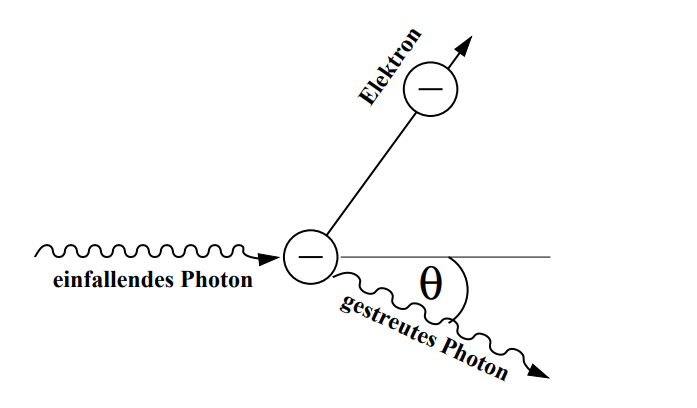
\includegraphics[scale=0.8]{content/Compton-Effekt.png}
    \caption{Die Streuung eines Photons an einem Elektron.\cite{sample}}
    \label{fig:CompPNG}
\end{figure}
\subsection{Bestimmung der Compton-Wellenlänge}
Um die Compton-Wellenlänge zu bestimmen wird die Transmisson und Absorbtion von Röntgenstrahlung durch Aluminium ausgenutzt.
Denn die Transmisson nimmt mit steigender Wellenlänge ab und demnach die Absorbtion zu. Entsprechend wird die Intesität der
einfallenden Welle $I_0$ nach dem Delamber'schen Gesetz
\begin{equation}
    I = I_0 e^{-\mu d}
\end{equation}
verringert. Dabei hat das absorbierende Material die Dicke $d$ und der Absorbtionskoeffizient $\mu$ setzt sich aus den Absorbtionskoeffizienten
der Paarbildung $\mu_{Paar}$, des Photoeffekts $\mu_{Photo}$ und des Comptoneffekts $\mu_{Com}$
\begin{equation*}
    \mu = \mu_{Paar} + \mu_{Photo} + \mu_{Com}
\end{equation*}
zusammen.
\subsection{Bragg'sche Reflexion}
Die Wellenlänge der Röntgenstrahlung $\lambda$ wird mithilfe der Bragg'schen Reflexion untersucht. Dabei fällt die Röntgenstrahlung auf ein dreidimensionales
Gitter(z.B. ein LiF-Kristall) und die Photonen werden dort an jedem Atom des Gitters gestreut. Die Röntgenstrahlung interferiert beim Glanzwinkel $\alpha$ konstruktiv
und es folgt die Bragg'sche Bedingung
\begin{equation}
    \label{eqn:Bragg}
    2d\sin\left(\alpha\right) = n\lambda.
\end{equation}
Hierbei ist $d$ die Gitterkonstante($d_{LiF} = \SI{201,4}{\pico\meter}$) und $n$ die Beugungsordnung.
